\section{Introduction}
In the 1950's, Solomon Asch performed a well-known series of experiments 
\cite{asch1956studies, asch1955opinions, bond1996culture} where
subjects were asked to choose which of a set of lines matched the
length of a reference line.  
When working individually, 99\% of the answers were correct.  
But when answering in the presence of a group of confederates who agreed on incorrect answers, 25\% of participants
conformed to the incorrect consensus.  
These results have been widely repeated to confirm what is now known as \emph{social influence bias}:
the tendency for participants to conform with the perceived community ``norm" \cite{demarzo2003persuasion,
moscovici1972social, wood2000attitude}.

Susceptibility to influence has been studied in the context of recommender systems \cite{cosley2003seeing}, and, in particular, Cosley et al. explored
different rating scenarios and how system-generated rating predictions may influence participant ratings.
They found that in a variety of scenarios including presenting manipulated predictions, presenting predictions on already rated items, and changing the rating scale had statistically significant influence on participants ratings.
The key conclusion of Cosley et al. is that rating and recommender systems are easily biased and they argue that these biases can mask a user's true
perception about a rated item.

\begin{figure}[t]
  \centering
    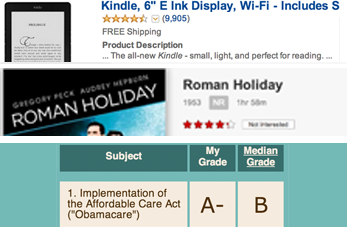
\includegraphics[width=\columnwidth]{../plots/intro2.png}
      \caption{Typical displays of aggregate prior rating values (the mean or median) in Amazon, Netflix, and the California Report Card
that has the potential to bias users.}
      \label{grading-0}
      \vspace{-1.0em}
\end{figure}

In almost all recommender systems, participants see the community ``norm" in the form of 
aggregate statistics (the average or median rating values) before entering a rating of their own;
potentially introducing social influence bias into the rating data.
This interface paradigm is, of course, reasonable to facilitate browsing and selection in a large lists of items.
For example, online retailers such as Amazon display the average rating value
for products and Netflix displays the average rating value of movies
(Figure \ref{grading-0}).  Display of average ratings values can also be
used as an incentive\cite{jian2012incentive} to reveal information about
peers after a participant enters his or her own grade.  
Display of statistics also increases the perceived transparency of open democracy platforms that encourage political engagement
\cite{albors2008new,o2012transparency,noveck2008wiki}.
Social influence bias can yield ratings that are closer to the average, less diverse, and less representative of participants' true
evaluations for items, which can in turn affect similarity measures between items and users and reduce the effectiveness of the recommendation system. 

In this paper, we propose a methodology to learn, analyze, 
and mitigate the effects of social influence bias in recommender systems.  
As a case study, we evaluate our methodology on a new recommender system, the 
California Report Card (CRC).
In the CRC, participants assign ratings (letter grades A+ to F, a 13 point
scale) to the State of California on six political issues.  
Then, the CRC uses the ratings to place participants in a open-ended
political discussion with an initial set of comments from those who 
rated the state most similarly.
Conformity ratings of the state can degrade the performance of the ``recommendation", 
a set of comments from like-minded participants.

The CRC has novel interface that allows us to learn the effects of Social Influence Bias.
The CRC interface reveals median grade values to participants \emph{after} they enter
their own rating and then allows participants to revise their
rating.
The key insight is that the combination of initial and revised ratings
pairs allows us to determine if the social influence bias is
statistically significant, and if so, can be used to build an
inference model that can predict the biasing tendency; thus mitigate the bias 
in a dataset of already biased ratings.  

Our methodology has three main components:
\vspace{1em}

\noindent \textbf{Learn} To initialize with baseline data, an initial
``learning" phase asks an initial set of participants to rate a set of
items twice: before seeing the median rating, and again after the
median is revealed.  This collects triplets of ratings for each
participant (initial rating, median rating, and final rating).

\vspace{1em}

\noindent \textbf{Analyze} Given these triplets, we propose a new
nonparametric significance test based on the Wilcoxon statistic to
determine whether ratings that were changed are significantly closer
to the median, i.e. the degree of social influence bias for each item.

\vspace{1em}

\noindent \textbf{Mitigate} Using the Bayesian Information Criterion
(BIC), we learn a polynomial function of optimal degree that estimates
the initial rating from the final rating and the median. This can be
used in a post-learning phase (when medians are always visible), or on
historical ratings, to estimate what a participant's rating would be
without social influence bias.

\vspace{1em}

A key priority is a nonparametric approach to modeling 
social influence bias. Many earlier studies of social influence
bias have focused on binary ratings (eg. up or down) \cite{muchnik2013social, zhu2012switch}.  
However, recommender systems often have multi-valued rating scales (eg. 5 stars).
Discrete multi-valued rating scales often exhibit multimodality and are not the optimal 
settings for parametric significance tests (eg. t-test and $\chi^2$ test).
In fact, it is known that a class non-parametric statistics called the Mann-Whitney statistics 
have far higher statistical power in these settings \cite{lehmann2006nonparametrics}, and
are further robust to outliers and long tails.
We use these results and properties to derive a new significance test for Social Influence Bias.

Not only is our testing framework nonparametric, but we also show that
we can relax assumptions about the structure of the social influence bias (eg. linear, conforming vs. contrarian).
We use the Bayesian Information Criterion to jointly optimize over the model parameters and the complexity hyperparameter in polynomial regression.
The result is a predictive model of social influence bias without having to make a strong assumption 
about the distribution of the data.

%estimate
%unbiased ratings and present results with data from the California
%Report Card, including learning curves that show that in most cases
%estimation converges relatively quickly.  Applying the proposed
%methodology to existing recommender systems raises a number of interesting
%questions for further research.

%In our case study, we apply this methodology to the California Report
%Card (CRC), a two-part recommender system that encourages political
%engagement.  In Part I, participants assign letter grades (a 13-point
%rating scale) to the state of California on six political issues.
%Part I uses the six ratings to quantify similarity between
%participants and issues.  In Part II, participants enter textual
%suggestions about new political issues and grade the suggestions of
%other participants.  Part II uses participant ratings to identify
%(recommend) valuable suggestions.  The CRC was announced via press and
%social media in late January 2014.

Results to date from the CRC suggest that given the opportunity, many
participants will revise their grades/ratings: $862$ out of $9390$
ratings were changed after participants saw the median value.  We
found statistically significant effects of social influence bias, with
ratings on average 19.3\% closer to the median value than ratings that
were not changed.  We also conducted an independent reference survey
using SurveyMonkey to ask a random sample of 611 participants from the
company's paid pool of California participants to grade the same set
of issues without displaying the median values.  This data did not
exhibit the same clustering around the median as the CRC, which
comparably had ratings that were statistically significantly closer to
the median (12.0\%), suggesting that social influence bias is an
important factor.

%We study social influence bias in this platform, especially since tendency to conform will affect our measure of similarity between participants in phase one.

%To minimize assumptions about the statistical distribution of ratings, we develop a non-parametric approach to test the following social influence hypotheses:

%\noindent \textbf{- Hypothesis 0} Given the opportunity, participants will revise their ratings.

%\noindent \textbf{- Hypothesis 1} When a participant does change a rating it will be in the direction that conforms to the presented median.

%\noindent \textbf{- Hypothesis 2} Participants will become more moderate in their ratings if they observe that their ratings consistently are in disagreement with the population consensus.

%Nearly 35\% of participants changed at least one rating, and our study finds statistically significant effects of social influence bias in the $862$ out of $9390$ ratings which were changed after participant's saw the median value.
%To further model patterns of participant behavior, we train a polynomial regression with the Bayesian Information Criterion (BIC) that predicts rating changes given a participant's current rating.
%The model can also be inverted to infer initial ratings from final ones.
%Prior results in social influence bias have focused on binary rating systems eg. up or down votes \cite{muchnik2013social, zhu2012switch}.
%However, these models are not directly applicable in many recommender systems which often have discrete mutli-valued rating scales (eg. 5 stars).

%Our results, which especially focus on mutli-valued ratings, have the following implications for interface and algorithmic design in recommender systems.
%Few existing tools collect both an initial (with the mean/median hidden) and a final rating.
%As seen in the CRC, given the opportunity to revise ratings, many participants will, and it can be informative to collect the pairs of ratings.
%The pairs can reveal more information about participants' initial perceptions, allow us to classify participants as likely to conform/deviate, and also assess the magnitude of social influence from the community.

%Existing recommender systems, can use our models to mitigate these effects, by training on set of rating pairs collected after-the-fact, and then applying the model to infer past participant's ``unbiased" ratings.

